\documentclass[a4paper]{ctexbook}

\usepackage{multirow}
\usepackage{booktabs}
\usepackage{enumitem}
\usepackage{CJK}
\usepackage[CJKbookmarks]{hyperref}  
\usepackage{listings} 
\usepackage{fancyhdr}
\usepackage{graphicx}

\hypersetup{%
	pdfstartview={FitH},% 文档初始视图为匹配宽度
	bookmarksnumbered={true},% 书签附上章节编号
	bookmarksopen={true},% 展开书签
	pdfborder=000,% 链接无框
	citecolor=blue,
	linkcolor=blue, % blue
	anchorcolor=blue,
	urlcolor=blue
}
\lstset{numbers=left, numberstyle=\tiny, stepnumber=1, numbersep=5pt,firstnumber=1,frame=shadowbox,columns=flexible,breaklines=true,language=csh}

\newcommand{\mvspace}{\vspace{0.5em}}
\newcommand{\inspace}{\hspace{2.5mm}}

\title{地震处理笔记 (SU和Madagascar)}
\author{孙波<seancug@cug.edu.cn>}
\date{created: 2017-06-11 \\ last updated: \today}


\begin{document}
	\maketitle
	\chapter*{序}
\addcontentsline{toc}{chapter}{序}
鄙人硕士学习期间接触过一段时间地震资料处理,对其方法原理以及流程略知一二。现今随波逐流于海洋物探采集,吾认为应当重拾地震处理,然专业软件非吾等贫民所能消费,因此以免费开源的SU(Seismic Unix)和Madagascar作替代。

本书即为SU和Madagascar学习笔记,其所收录之内容,或个人总结,或来自于网络上摘录,或来自某日某时于某书上发现之有价值之内容,林林总总,无论出自自己或他人,但凡本人有兴趣者,皆收入本书中。本书无终成之日,但随心而已,无论何时何地,兴之所致,皆可添加新内容。
	\tableofcontents
	
	\part{Seismic Unix}
	\chapter{地震数据基本操作}
\section{获得帮助}


\begin{enumerate}
	\item[suhelp] 显示可执行的程序和Shell脚本。
	\item[suname] 列出SU中各项命令的名字和简短描述,以及编码的地址。
	\item[sudoc] 得到编码的DOC列表,列出SU中各条目的在线文档。更加具体
	\item[sufind] 在自述文档中得到信息,使用给定的字符串查找SU命令。
	\item[Demo] SU软件包中有一套Shell脚本演示程序。
	放在目录CWPROOT/src/demos,CWPROOT/src/demos/README文件是这些演示程序的说明书。
	Making Data 演示程序显示使用susynlv程序制作合成记录炮集和共偏移距道集的基础内容。应当特别注意演示中好的标注风格。
	Filter/Sufilter 使用实际数据处理例子演示说明消除地滚波和初至。
	Deconvolution 使用supef和其它工具简单合成脉冲道集来实例说明去混响和脉冲反褶积处理。演示程序包括使用loops系统检验滤波参数影响的命令。
	\item[sukeyword] 列出SU道头中的关键字  sukeyword –o
	\item[基本用法] SU基本用法是通过创建Shell脚本来实现相应的数据处理。su/examples目录下有很多这样的例子。   
\end{enumerate}   


\section{道头操作}
SU数据格式继承了SEGY的道头。如果你的数据不是SEGY,而是从其它格式转换得到的,就需要设置一些道头关键字,以使得数据与SU程序协调一致。\\
\begin{tabular}{lp{0.7\textwidth}}
	\toprule
	suaddhead & 在裸数据中写道头,设置道头字\\
	sustrip & 把SU格式数据中的道头切除并存放在文件中,形成裸数据\\
	supaste & 把道头文件再粘贴回来,把裸数据添加道头文件生成SU格式的数据文件\\
	sukeyword & 文件“segy.h”中SU的关键字指南\\
	surange & 获得非零道头输入值的范围(最大值和最小值)\\
	sushw & 设置一个或多个道头字,利用道数、取余数(mod)或整除(integer divide)计算道头字的值,或从一个文件中输入道头字的值\\
	suchw & 利用一个或两个已存在的道头字来计算新的道头字	\\
	sugethw & 获取SU数据中道头字的值\\
	suedit & 检查Segy磁盘文件并编辑道头\\
	suxedit & 检查Segy磁盘文件并编辑道头\\	
	suswapbytes & 把SU数据字节顺序从big endian交换为little endian,或者是相反\\
	\bottomrule
\end{tabular}

\begin{table}[h]
	\centering
	\begin{tabular}{ll}
		\toprule
		Key & Definition \\
		\midrule
		dt &  采样率 microseconds \\ 
		ns &  一道中采样数 \\
		ntr & 道数 \\
		offset & 偏移距 \\
		tracf & 炮集中道号 field record (gather) \\
		tracl & 测线中的道号 line \\
		tracr & 整个数据中道号 reel (entire data set) \\
		delrt & 延迟时间 milliseconds \\
		fldr  & 记录炮集号 field record number\\
		\bottomrule
	\end{tabular}\\
	\caption{常见关键字}                   
\end{table}

\begin{enumerate}
	\item[suaddhead] suaddhead – 给二进制数据加SU道头 \par
	如果我们的数据由二进制C浮点型文件组成(例如每道1024个采样点),那么下面命令系列将产生SU数据文件“data.su”:\par
	\framebox[0.8\textwidth]{suaddhead < data.bin ns=1024 > data.su\hfill}\par
	对于其它类型(如整型)使用命令recast:
\begin{lstlisting}[language=python]
recast < data.ints in=int out=float | suaddhead ns=1024 > data.su\hfill}
\end{lstlisting}
	如果数据首先是从Fortran转换而来的整型,那么处理流程为:
\begin{lstlisting}[language=python]
ftnstrip < data.fortran | recast in=int out=float | suaddhead ns=1024 > data.su\hfill}\par
\end{lstlisting}
	\item[sustrip] 将SU道头与SU数据分离\par
	命令suaddhead的逆操作就是sustrip.下面的命令行将去掉文件SU道头,并把SU道头存到“data.headers”中,形成裸数据data.bin:\par
	\framebox[0.8\textwidth]{sustrip < data.su head=data.headers > data.bin\hfill}
	\item[supaste] 将SU道头与SU数据合成\par
	对二进制数据完成处理后,我们可能需要把道头粘贴回去,这时用命令supaste。下面的命令行将把文件“data.headers”中的道头内容粘贴回数据中:\par
	\framebox{supaste < data.bin head=data.headers > data.su}\par
	\framebox{supaste < data.bin head=data.headers > data.su}\par sukeyword – \item[sukeyword] 查看SU关键字 sukeyword -o\par
	将显示SU关键字的列表,SU道头中确定有80多个关键字,大多时候只使用其中相对很小的一部分。
	\item[surange] 获得道头字值的范围\par
	指定数据中道头字值得范围,对于道头字而言是非常有用的信息。键入:\par
	\framebox{surange < data.su}\par
	将返回所有非零SU道头字值得范围。\par
	请注意,对于损坏的数据来说,很多道头字中可能出现非常奇怪的值,检测这种问题也是surange命令的主要用法之一。
	\item[sugethw] 获取SU道头字的值\par
	surange命令可以查看整个数据道头字的范围(最大值和最小值)。但是,我们往往需要按一定的顺序一道一道地查看道头字的值。命令sugethw就是这样的一个工具。例如:\par
	\framebox{sugethw < data.su key=keyword1,keyword2,... | more}\par
	下面给出一个具体的例子:\par
	\framebox{suplane | sugethw key=tracl,tracr,offset,dt,ns | more}\par
	sugethw对于道头字的排列顺序和个数没有要求,但至少要指定一个道头字。\par
	如果需要把道头字输出成二进制的文件,可用下面的命令:
\begin{lstlisting}[language=python]
suplane | sugethw key=tracl,tracr,offset,dt,ns output=binary > file.bin}
\end{lstlisting}
	对于观测系统,你可以使用下面的命令输出到文件中去:
\begin{lstlisting}[language=python]
suplane | sugethw key=tracl,tracr,offset,dt,ns output=geom > hdrfile}
\end{lstlisting}
	\item[sushw] 在SU数据中设定道头字的值\label{key:sushw}\par
	命令sushw可根据各种需要来设置道头字的值,该命令可以一次让用户设置一个或多个道头字的值。使用sushw对道头字指定一个固定的值,如我们给数据设定采样间隔:\par
	\framebox{sushw < data.su key=dt a=2000 > data.out.su}\par\vspace{0.5em}
	\begin{tabular}{ll}
		\toprule
		\multicolumn{2}{l}{sushw指定的可选参数有:}\\
		\midrule
			key & 要修改的关键字\\	
			a & 第一道的值\\		
			b & 组内增加量\\			
			c & 组间增加量\\			
			d & 道偏移量\\			
			j & 组内元素个数\\
		\bottomrule
	\end{tabular}\par\vspace{0.5em}
	sushw指定的可选参数有:\par
	这些额外的可选参数可用来做更加复杂的操作。这样做是非常重要的,因为道头字的值与道数据的位置常常有直接的关系。道头字的值用下面的公式计算:
	$$i = itr + d$$
	$$val(key) = a + b *  \left( i \% j\right)   + c * \left( i / j \right) )$$
	这里itr是道号(注意:第一道是itr=0,而非1),\%表示取余数,/表示除法。\par
	例如,我们可以设定头五道的道头字sx=6400,第二个5道中sx=6300,依次类推,每5道递减100:\par
	\fbox{sushw < data.su key=sx a=6400 c=-100 j=5 > data.new.su}\par
	另一个例子,我们设置每5道的offset的值为200:200:1000,命令格式为:\par
	\fbox{sushw < data.su key=offset a=200 b=200 j=5 > data.out.su}\par
	我们可以只使用一个sushw命令就可以完成上面3个操作:
\begin{lstlisting}[language=python] 
sushw < data.su key=dt,sx,offset a=2000,6400,200 b=0,0,200 c=0,-100,0 j=0,5,5 > newdata.su
\end{lstlisting}
	下面是一个实际的例子,tracl从1开始,每隔100道增加1;cdp从1开始,每道增加1,一直增加到100,然后重复从1开始;offset同tracl,只是从0开始;sx同cdp;sy同offset;ns全部设为495;dt全部设为1000:
	\begin{lstlisting}[language=python] 
sushw < filename.su key=tracl,cdp,offset,sx,sy,ns,dt a=1,1,0,1,0,495,1000 b=0,1,0,1,0,0,0 c=1,0,1,0,1,0,0 j=100,100,100,100,100,0,0 > filename_new.su
	\end{lstlisting}
	\item[suchw] 在SU数据中改变(或计算)道头字的值\par
	有些道头字(如cdp)可以从已有的道头字计算而来,程序suchw就提供了这种功能。\par
	参数有:\par
	\begin{tabular}{ll}
		\toprule
		key1 & 输出的关键字\\
		key2 & 输入的关键字\\
		key3 & 输入的关键字\\
		a & 偏移量\\
		b & key2关键字的倍数\\	
		c & key3关键字的倍数\\	
		d & overall scales\\
		\bottomrule
	\end{tabular}\par
	我们可以使用两个道头字的值(key2和key3),利用下面的方程式计算第三个道头字的值(key1):\par
	\fbox{val(key1) = (a + b * val(key2) + c * val(key3)) / d}\par
	例如:\par
	suchw<indata key1=gx,cdp key2=offset,gx key3=sx,sx b=1,1 c=1,1 d=1,2 >outdata
	\item[suedit和suxedit] 编辑SU数据中道头字的值\par
	最后,你可能想检查或改变某个道头,suedit和suxedit命令就可以提供这个功能。允许交互浏览和编辑道头字。\par
	例如:\\
	\fbox{suplane > data.su}\\
	\fbox{suedit data.su}\\
	将得到下面的结果:\\
	\begin{tabular}{|l|}
		\toprule
		32 traces in input file\\
		tracl=32 tracr=32 offset=400 ns=64 dt=4000\\
		>  prompt for interactive use\\
		\bottomrule
	\end{tabular}\\\\
	suedit 和suxedit交互使用的命令可以通过在提示符后键入问号(?)显示。例如:\\
	\begin{tabular}{|l|}
	\toprule
	32 traces in input file\\
	tracl=32 tracr=32 offset=400 ns=64 dt=4000\\
	>?\\
	n  read in trace \#n\\
	<CR>   step	\\
	+    next trace;\\ 	
	step -> +1\\	
	-  prev trace;  \\  	
	........\\
	\bottomrule
	\end{tabular}\\\\
	该程序让用户将数据采样值按表格形式浏览到数据,或者浏览或改变单个道头字的值。\\
	程序suxedit和suedit类似,但含有X-Wi
\end{enumerate}             
     

\section{数据读写}

\begin{tabular}{lp{0.48\textwidth}}
	\multicolumn{2}{c}{从磁带上读写数据}\\
	\toprule
	\multicolumn{2}{p{0.9\textwidth}}{下面的程序对于地球物理应用中特定的数据输入和输出任务是有用的,对内部SU数据格式也一样}\\
	\midrule
	bhedtopar & 把二进制磁带HEaDer文件转换成PAR文件格式\\
	dt1tosu &  把Sensors,Software X.dtl GPR的地质雷达数据转成SU格式\\
	segdread & 读取SEGD磁带\\
	segyclean & zero out unassigned portion of header\\
	segyread & 读SEGY磁带\\
	segyhdrs & 为segywrite构造SEGY文件的ascii和二进制头文件SEGYWRITE写SEGY磁带\\
	setbhed & 设置一个SEGY二进制磁带HEaDer文件的道头字\\
	suaddhead & 为裸道加上头文件并设置tracl和ns道头字\\
	sustrip & 从道中去掉SEGY头文件\\
	supaste & 为已存在的数据加上已存在的SEGY头文件\\
	\bottomrule	
\end{tabular}\par
\mvspace
\begin{enumerate}
	\item[SEGY/SU] SEGY格式和SU数据格式\par
	SEGY数据格式包括三个部分:\par
	第一个部分是3200字节的EBCDIC卡片,包括40个卡片(等于每行包含80个字符的40行文本),用来磁带。\par
	第二个部分时400个字节的二进制头文件,含有磁带卷内容的信息。\par
	第三个部分是真正的地震道数据。每道有240个字节的道头文件。接下来,是32位的IBM浮点型数据(在IBM Form GA 22-6821中定义)。注意,IBM格式和现代IBM PC上所用的IEEE格式是不同的。\par
	SU数据格式是基于SEGY格式的道部分。SEGY道和SU道的主要不同在于SU格式的道数据是浮点型,是和你运行SU程序的计算机上的浮点格式一致的。SU数据只含有SEGY的道部分!SU格式中不保存EBCDIC和二进制卷头,所以无法在任何SU程序中直接使用SEGY文件。\par
	为了把SEGY数据转成SU程序所用的格式,需要使用segyread。
	
	\item[segyread] 将SEGY数据读入SU\par
	程序segyread用来把数据从SEGY格式转成SU格式。当读取SEGY磁带或数据文件时,你需要知道你所使用的机器的byte-order(“big-endian”或“little-endian”)。\par
	在big-endian机器上运行segyread的典型方式如下所示:
\begin{lstlisting}[language=python] 
segyread tape=/dev/rmt0 verbose=1 endian=1 > data.su\hfill}\par\mvspace
\end{lstlisting}
	更经常使用的是如下的格式来为big-endian平台读入数据:\par
\begin{lstlisting}[language=python] 
segyread tape=/dev/rmt0 verbose=1 endian=1 | segyclean >data.su\hfill}\par\mvspace
\end{lstlisting}
	在SEGY道头里有可选的道头字(字节181-240)。这些道头字的使用没有标准,所以很多人按自己的需要来填写。SU也不例外。有几个SU图形程序使用的参数存储在这些道头字里。程序segyclean会把可选道头字里容易让SU图形程序产生误解的参数清零。\par
	糟糕的是有很多号称SEGY格式,但却不符合SEG的标准SEGY格式。最常见的情况就是为了方便,道部分是用IEEE格式。这种IEEE格式数据可用下面的命令来读取:\par
\begin{lstlisting}[language=python]
segyread tape=/dev/rmt0 verbose=1 endian=1 conv=0 | segyclean > data.su\hfill
\end{lstlisting}
	这里conv=0是告诉程序不进行IBM型到float浮点型的转换。还有DOS SEGY格式,基本与前面相同,除了他的道和头都是用little-endian格式写的。如果用big-endian机器来读的话用下面的命令:\par
\begin{lstlisting}[language=python]
segyread tape=/dev/rmt0 verbose=1 endian=0 conv=0 | segyclean > data.su
\end{lstlisting}
	注意:endian=0是设置交换字节(所有的字节,头和数据都是交换格式)。在little-endian机器上,程序是:\par
\begin{lstlisting}[language=python]
segyread tape=/dev/rmt0 verbose=1 endian=1 conv=0 | segyclean > data.su
\end{lstlisting}
	endian=1会阻止交换字节。不管哪种情况,如果我们的磁盘文件名为“filename”,那么应该使用“tape=filename”参数。
	
	\item[segywrite]  写SEGY格式的磁带或磁盘文件\par
	与segyread相对应的命令是segywrite。这个程序可以将SEGY格式按多种不同的方式把数据写到磁带或磁盘文件。该程序可用于把数据写成商业软件可以使用的形式。在学习如何使用segywrite命令之前,有几个需要的准备步骤必须要讨论一下。
	
	\item[segyhdrs] 为segywrite准备ascii和二进制头文件。\par
	要写一个符合SEG数字磁带标准的SEGY格式,你需要提供ASCII和二进制的卷头文件,在SEGY磁带或文件里会变成EBCDIC和二进制的卷头文件。也就是segywrite创建文件时需要有header部分和binary部分。\par
	如果你没有binary和header文件,你必须用程序sgyhdrs(创建SEG Y文件)来创建它们。命令:\par
	\framebox[0.9\textwidth]{segyhdrs < data.su\hfill}\par\mvspace
	会在当前工作目录下写header和binary文件。
	文件header是一个ASCII文件,可以用正常的文本编辑器来编辑。可以放任意内容,只有格式是每行80个字符的40行。Segywrite会自动把segyhdrs产生的缺省头文件转成下面的格式:\par
	\mvspace
	\begin{tabular}{|l|}
		\hline
		C This tape was made at the\\
		C\\
		C Center for Wave Phenomena\\
		C Colorado School of Mines\\
		C Golden, CO, 80401\\
		C\\
		...\\
	   \hline
	\end{tabular}
	\item[bhedtopar] 编辑二进制头文件\par
	要编辑二进制头文件,首先要转成ASCII格式。程序bhedtopar允许把binary文件写成“parfile”的格式:\par
	\framebox[0.9\textwidth]{bhedtopar < binary outpar=binary.par\hfill}\par\mvspace
	可以编辑产生的ASCII码文件“binary.par”进行修改,然后通过setbhed来重新读入:\par
	\framebox[0.9\textwidth]{setbhed bfile=binay par=binary.par\hfill}\par\mvspace
	也可以单独设置头文件字。例如:\par
	\framebox[0.9\textwidth]{setbhed bfile=binary par=binary.par lino=3\hfill}\par\mvspace
	使用了binary.par的内容,但是lino单独设为3。最后,可以通过下面的命令来写磁带:\par
	\framebox[0.9\textwidth]{segywrite tape=/dev/rmtx verbose=1 < data.su\hfill}\par\mvspace
	注意header文件和binary文件是在当前目录下的。你也可以使用你自己的文件名。Segywrite的选项bfile=和hfile=用来输入你指定的文件名。
\end{enumerate}


\section{数据格式转换}
\begin{tabular}{ll}
	\multicolumn{2}{c}{一般数据输入}\\
	\toprule
	\multicolumn{2}{p{0.9\textwidth}}{下面的程序可以用于一般的数据输入,输出和数据格式转换,在磁带读写中也可以使用。}\\
	\midrule
	a2b & 把ascii float转成二进制\\
	b2a &把二进制float转成ascii\\	
	ftnstrip & 把Fortran的float转成C格式的float\\	
	h2b & convert 8 bit hexidecimal floats to binary\\	
	recast & 改变数据类型(从一种数据类型转到另一种)\\	
	transp & 转置一个n1×n2个元素的矩阵\\
	\bottomrule
\end{tabular} 

\begin{enumerate}
	\item[a2b和b2a] ASCII to Binary, Binary to ASCII\par
	在所有的数据格式中,ASCII是最常传送的(也是最耗空间的)。不管你使用什么系统,都可能需要把ASCII转来或转去。而且,因为文本编辑器支持ASCII,因此经常可能要用文本编辑器来做数据输入或编辑。\par
	这种格式大都是多行格式,用空格或tab来隔开。要转换一个例如5行的数据到二进制,键入:\par
	\framebox[0.9\textwidth]{a2b < data.ascii n1=5 > data.binary\hfill}\par
	相反的操作就是:\par
	\framebox[0.9\textwidth]{b2a < data.binary n1=5 > data.ascii\hfill}\par
	\item[ftnstrip] 把Fortran数据转换成C语言格式\par
	Fortran在地震数据处理中是比较流行的语言,因此常常需要处理Fortran创建或处理过的数据。Fortan的二进制数据是被beginning-of-record和end-of-record分隔符隔开的。而C程序创建的二进制数据没有这些分隔符。要在C程序中使用Fortran数据需要去掉这些Fortran标签,通过:\par
	\framebox[0.9\textwidth]{ftnstrip < fortdata > cdata\hfill}
	\item[recast] 改变数据类型(从一种数据类型转到另一种)\par
	float 浮点型, double 双精度, int (带符号)整型, char 字符, uchar 无符号字符, short 短整型, long 长整型, ulong 无符号长整型\par
	例如,把整型转换成浮点型:\par
	\framebox[0.9\textwidth]{recast < data.ints in=int out=float > data.floats\hfill}
	\item[transp] 转置一个n1×n2个元素的矩阵
	\item[farith] 对二进制数据作简单的算术运算\par
	很多时候需要对文件做算术操作,或者在两个二进制数据文件之间。程序farith用来完成许多类似的任务.\par
    \mvspace
	Farith对单个文件的操作包括:\par
	\rule{0.9\textwidth}{0.1em}\\
	Scaling value(缩放数值)\par
	Polarity reversal(极性反转)\par
	Signum function(正负号函数)\par
	absolute value (绝对值)\par
	exponential(取指数)\par	
	logarithm(取对数)\par	
	square root (开平方根)\par
	square(取平方)\par
	inverse (punctuated), (取道数,带小数点)\par
	inverse of square (punctuated), (取平方倒数,带小数点)\par
	inverse of square root (punctuated) (取平方根倒数,带小数点)\par
    \vspace{0.6cm}
	二元操作(对两个文件的操作)包括\par
	\rule{0.9\textwidth}{0.1em}\\
	addition (加法)\par
	subtraction  (减法)\par
	multiplication (乘法)\par
	division  (除法)\par
	Cartesian product笛卡尔乘积:从给定的集合X和Y中构成的所有(x,y)元素对集合\par
	\vspace{0.6cm}
	地震操作包括\par
	\rule{0.9\textwidth}{0.1em}\\
	slowness perturbation\par
	sloth perturbation\par
	\vspace{0.4cm}
	使用farith的实例:\par
	\framebox[0.9\textwidth]{farith in=data.binary op=pinv out=data.out.bin\hfill}\par
	\framebox[0.9\textwidth]{farith in=data1.binary in2=data2.binary op=add > data.out2.bin\hfill}
\end{enumerate}                  
                
   
                 
   

	\chapter{SU数据常用操作}
\section{编辑SU数据}
一旦SU格式的数据读入和道头设置正确后,常常要对数据进行操作和编辑。SU提供的数据处理和编辑的命令有\ref{table:here}:\par\mvspace
\begin{tabular}{lp{0.65\textwidth}}
	\toprule
	suwind & 根据关键字开时窗\\	
	susort & 基于segy道头关键字进行道分选\\	
	suramp & 从道起点到道终点进行线性斜坡化(Linearly taper)至零值\\	
	sutaper & 对一个数据窗进行斜坡化(taper)至零值\\	
	sunull & 产生空道(都为零值)\\	
	suzero & 在一时间窗内数据充零\\	
	sukill & 地震道充零\\	
	sunute & 根据关键道头字确定的距曲线的距离,去除用户指定的多边形曲线上边或下边的值\\	
	suvlength & 调整变长度地震道到相同长度地震道\\	
	suvcat & 将一个数据附加到另一个数据(一道接一道进行)\\
	\bottomrule
	\label{table:here}
\end{tabular}

\begin{enumerate}
	\item[suwind] 用关键字选定一定时窗地震道\\
	非常常见的操作就是我们时常需要浏览或处理地震数据中的一小块数据。suwind命令使得我们可以根据大量的参数信息设置窗口来选定感兴趣的数据。\par\mvspace
	\fbox{通过道头字来设定数据窗口的大小}\par
	suwind最简单的用法就是,通过用户设定道头关键字的最小和最大值来选定数据:\\\\
	\begin{tabular}{ll}
		\toprule
		key=tracl & 设置窗口的道头字(see segy.h)\\
		min=LONG\_MIN &   数据关键道头字的最小值\\
		max=LONG\_MAX &   数据关键道头字的最大值\\
		\bottomrule
	\end{tabular}\\\\
	例如,用道数作关键字对命令suplane产生的数据进行窗口大小设置:
\begin{lstlisting}[language=python] 
suplane | suwind key=tracl min=5 max=10 | sugethw key=tracl | more
\end{lstlisting}
	对于一个大的数据体,应该使用计数(count)参数,而不是最大值。如果直接设定最大值(max),命令suwind将查询全部数据后,再选择在最小值和最大值之间的道集,这是因为程序认为道的标志(trace labeling)可能多次出现。例如,可以比较下面的两个命令的结果:\\
\begin{lstlisting}[language=python] 
suplane ntr=100000 | suwind key=tracl min=5 max=10 | sugethw tracl | more	
suplane ntr=100000 | suwind key=tracl min=5 count=5 | sugethw tracl | more
\end{lstlisting}	
	更复杂的窗口大小选择如下(例如,使用分数,decimating data):\par
	\mvspace
	\begin{tabular}{ll}
		\toprule
		j=1 & 通过每个j道…	\\
		s=0 & 以s为基数(如果((key - s)\%j) == 0) \\
		\bottomrule
	\end{tabular}\par
	\mvspace
	下面的例子用suplane生成的数据,每两道抽取一道(即抽取道2、4、6…):
\begin{lstlisting}[language=python]
suplane | suwind key=tracl j=2 | sugethw key=tracl | more
\end{lstlisting}	
	或者每隔2道抽取1道,基数为1(即抽取道1、3、5…):
\begin{lstlisting}[language=python]	
suplane | suwind key=tracl j=2 s=1 | sugethw key=tracl | more
\end{lstlisting}	
	也可以用suwind接受或拒绝某些地震道:\par
	\mvspace
	\begin{tabular}{ll}
		\toprule
		reject=none  &   按指定的关键字跳过的地震道\\
		accept=none   &   用指定的关键字选择地震道\\
		\bottomrule
	\end{tabular}\par
	\mvspace
	例如下面的命令所示,地震道中的第3、8、9道将不显示:
\begin{lstlisting}[language=python]		
suplane | suwind key=tracl reject=3,8,9 | sugethw key=tracl | more
\end{lstlisting}	
	参数accept选项有点特殊,它表示接收这些道,即使这些道被拒绝过。例如:
\begin{lstlisting}[language=python]	
suplane | suwind key=tracl reject=3,8,9 accept=8 | sugethw key=tracl | more
\end{lstlisting}	
	如果你只想接收列表中的道,这时需要设置参数“max=0”,下列所示只显示出第8道:
\begin{lstlisting}[language=python]	
suplane | suwind key=tracl accept=8 max=0 | sugethw key=tracl | more
\end{lstlisting}	
	计数(count)参数覆盖接收(accept)参数,所以如果你想真正无条件接受道,就不能指定计数(count)参数。\par
	\mvspace
	\fbox{选取时间窗口(Time gating)}\\
	有关窗口的第二个问题就是时间窗的设定。垂直时间窗(time gating)的选项为:\\
	\begin{tabular}{ll}
		\toprule
		tmin = 0.0 & 选取最小时间	\\
		tmax = (from header) &  选取最大时间	\\
		itmin = 0 & 选取最小时间采样\\	
		itmax = (from header) & 选取最大时间采样\\	
		nt = itmax-itmin+1 & 时间采样点数	\\
		\bottomrule
	\end{tabular}\par
	\mvspace
	设置的结果要么是选取最小时间采样和选取最大时间采样(itmin和itmax),要么选取最小时间和选取最大时间(tmin和tmax),这样就将产生一个最接近采样的时窗。
	\item[susort] 根据segy道头字分选道\\
	susort命令利用Unix系统sort命令,通过道头关键字对地震道进行分选。\\
	例如,根据两个关键字(cdp和offset)分选数据(数值按升序),可用下面的命令:
\begin{lstlisting}[language=python]	
susort <indata.su >outdata.su cdp offset
\end{lstlisting}
	如果offset关键字按降序,cdp关键字按升序进行分选,可用下面的命令:
\begin{lstlisting}
susort <indata.su >outdata.su cdp -offset
\end{lstlisting}
	
	\item[suramp和sutaper] 数据斜坡化(Tapering)
	很多地震处理算法因为数据的突变边界而显示假象,在数据边界对振幅进行斜坡化(tapering),就是压制这种假象的最容易的方法。在SU中,我们可以使用sutaper命令对数据边界进行斜坡化。\\
	例如,对每5道数据从头到尾进行斜坡化:
\begin{lstlisting}
sutaper <diskfile >stdout ntaper=5
\end{lstlisting}
	suramp可以平滑从起始道和(或)末道。例如,斜坡化从0到tmin=0.05s,然后再向下从tmax=1.15s到末道:
\begin{lstlisting}
suramp <diskfile tmin=.05 tmax=1.15 >stdout
\end{lstlisting}
	\end{enumerate}\par
	sukill、suzero、sunull和sumute– 数据充零\par
	对有噪声的道、位于数据边界的道进行充零是有益的。或者是产生一些空道,在绘图时最为联系数据集中间的分割标志。

\begin{enumerate}
	\item[sukill] 道充零
\begin{lstlisting}
sukill <stdin >stdout min=MIN_TRACE count=COUNT
\end{lstlisting}
	这里参数count是要充零的总道数,参数min是要充零的这些道中的最小道号。
	\item[sunull] 产生空道数据\\
	有时需要生成道值为零的地震数据块。下面的命令产生共有NTR道,时间采样数为NT的地震数据:
\begin{lstlisting}
sunull nt=NT ntr=NTR <stdin >stdout min=MIN_TRACE count=COUNT
\end{lstlisting}	
	\item[suzero] 在一段时间窗内对数据充零
\begin{lstlisting}
suzero itmin=MIN_TIME_SAMPLE itmax=MAX_TIME_SAMPLE <indata.su > outdata.su
\end{lstlisting}
	\item[sumute] 数据去除	
	要进行高精度的压制操作,可用命令sumute对SU数据进行处理。
\begin{lstlisting}
sumute <indata.su >outdata.su key=KEYWORD xmute=x1,x2,x3,...tmute=t1,t2,t3,...
\end{lstlisting}
	下面用suplane生成数据,然后做去除处理与原始生成数据比较:
\begin{lstlisting}
suplane | suxwigb 
suplane | sumute key=tracl xmute=1,10,12 tmute=.06,.1,.11 | suxwigb 
\end{lstlisting}
	去除根据xmute=和tmute=参数确定的多边形曲线内每一个初至。
	\item[suvcat和cat] 数据合并\\
	有两种方法可以将一种数据附加到另一个上(合并)。第一种使用Unix命令cat,简单的将第二个文件的数据放到第一个文件中去。
\begin{lstlisting}
cat data1.su data2.su > data3.su
\end{lstlisting}	
	另外,可能需要对地震道重编号:
\begin{lstlisting}
cat data1.su data2.su | sushw key=tracl a=1 > data3.su
\end{lstlisting}	
	第二种是将第二个数据集中的每一道垂直的附加到第一个数据集中每一道的末尾。这就需要使用suvcat命令:
\begin{lstlisting}
suvcat data1.su data2.su > data3.su
\end{lstlisting}
	在这个例子中,就不需要修改道头字。
	\item[suvlength] 调整可变长度道到相同采样点数	\\
	有时数据中每道含有不同的采样点数。下面我们对用suplane命令生成的数据,用命令suvlength处理的道相同的采样点数:
\begin{lstlisting}
suplane nt=64 > data1.su
suplane nt=32 > data2.su	
cat data1.su data2.su > data3.su
\end{lstlisting}
	对于上面合并生成的数据data3.su,如果想用SU程序处理该数据文件将会失败,因为大多说SU程序要求数据块含有相同的采样点数。使用命令suvlength可以解决该问题:
\begin{lstlisting}
suvlength ns=64 < data3.su > data4.su
suxwigb < data4.su title="Test of suvlength" 
\end{lstlisting}	
	这将使所有的道含有相同的长度。
\end{enumerate}

\section{SU数据常用操作}
\begin{tabular}{ll}
	\toprule
	suaddnoise – 对地震道加噪声\\
	sugain – su数据增益\\
	suop – su数据的一元操作\\
	suop2 – su数据的二元操作\\
	\bottomrule
\end{tabular}
\begin{enumerate}
	\item[suaddnoise] 对地震道加噪声\\	
	下面是两个使用suaddnoise命令的例子:
\begin{lstlisting}
suplane | suxwigb title="no noise" 
suplane | suaddnoise | suxwigb title="noise added" 
suplane | suaddnoise sn=2 | suxwigb title="noise added" 
\end{lstlisting}
	\item[sugain] su数据增益
	增益命令含有多个选项:\par\vspace{0.1em}
	\begin{tabular}{p{0.42\textwidth}p{0.42\textwidth}}
	\toprule
	scaling the data & 数据比例伸缩\\
	multiplying the data by a power of time & 数据与时间幂相乘\\
	taking the power of the data & 数据取幂\\
	automatic gain control & 自动增益控制\\
	trapping noise spiked traces & 含噪声脉冲的地震道陷波滤波\\
	clipping specified amplitudes or quantiles & 指定的振幅或分量裁减限制\\
	balancing traces by quantile clip, rms value, or mean &根据等分法、均方根值或均值道均衡\\
	biasing or debiasing the data & 偏离或去偏离数据 \\
	\bottomrule
	\end{tabular}\par\mvspace
	操作优先等级如下面的方程所示:
	$$out(t) = scale*bal\left\lbrace clip\left[ agc\left\lbrace \left[ t^{tpow}*e^{epow*t}*\left( in(t)-bias\right) \right] ^{gpow}\right\rbrace \right] \right\rbrace )$$
	实例:
\begin{lstlisting}
suplane | suaddnoise > data.su
suxwigb < data.su title="Ungained Data" 	
sugain < data.su scale=5.0 | suxwigb title="Scaled data" 	
sugain < data.su agc=1 wagc=.01 | suxwigb title="AGC=1 WAGC=.01 sec 	
sugain < data.su agc=1 wagc=.2 | suxwigb title="AGC=1 WAGC=.1 sec 	
sugain < data.su pbal=1 | suxwigb title="traces balanced by rms" 
sugain < data.su qbal=1 | suxwigb title="traces balanced by quantile" 	
sugain < data.su mbal=1 | suxwigb title="traces balanced by mean" 	
sugain < data.su tpow=2 | suxwigb title="t squared factor applied" 	
sugain < data.su tpow=.5 | suxwigb title="square root t factor applied" 
\end{lstlisting}
	\item[suop] su数据的一元操作\\ 
	suop对SU数据进行一元函数运算和操作,主要功能包括:\par
	\begin{tabular}{p{0.45\textwidth}l}
		\toprule
			absolute value & 取绝对值	\\		
			signed square root & 带符号开方\\		
			square & 平方	\\		
			signed square & 带符号位平方\\			
			signum function & 正负号函数	\\		
			exponential & 指数\\			
			natural logarithm & 取自然对数\\			
			signed common logarithm & 带符号位常用对数	\\		
			cosine & 余弦函数\\			
			sine & 正弦函数	\\		
			tangent &  正切函数	\\		
			hyperbolic cosine &  双曲余弦函数	\\		
			hyperbolic sine & 双曲正弦函数\\			
			hyperbolic tangent & 双曲正切函数	\\		
			divide trace by Max. Value & 地震道数据用最大值除	\\		
			express trace values in decibels: 20 * slog10 (data) & 地震道数据用分贝表示\\			
			negate values & 数据取反\\			
			pass only positive values & 只选正值\\			
			pass only negative values & 只选负值\\
			\bottomrule
	\end{tabular}\\\\
	例子:
\begin{lstlisting}
suplane | suaddnoise > data.su
suop < data.su op=abs | suxwigb title="absolute value" 	
suop < data.su op=ssqrt | suxwigb title="signed square root" 	
suop < data.su op=sqr | suxwigb title="signed square" 	
\end{lstlisting}
	
	\item[suop2] su数据的二元操作
	程序suop2用来对两个SU数据进行操作,该命令支持的计算有:\par
	\begin{tabular}{p{0.45\textwidth}l}
		\toprule
		difference &  相减\\
		sum & 相加\\	
		product & 相乘\\	
		quotient & 相除\\
		\bottomrule
	\end{tabular}\\\\
	前面的选项假定每个SU数据道采样数相同,后面4个选项假定第二个文件只有一道。\par
	\begin{tabular}{p{0.45\textwidth}l}
		\toprule
		difference of a panel and a single trace & 一块数据和某一道数据相减\\
		sum of a panel and a single trace & 一块数据和某一道数据相加\\
		product of a panel and a single trace & 一块数据和某一道数据相乘\\
		quotient of a panel and a single trace & 一块数据和某一道数据相除\\
		\bottomrule
	\end{tabular}\\\\
	并且有8个对等shell文本命令做这些操作:\\
	\begin{tabular}{ll}
		\toprule
		susum file1 file2 & suop2 file1 file2 op=sum\\
		sudiff file1 file2 & suop2 file1 file2 op=diff\\	
		suprod file1 file2 & suop2 file1 file2 op=prod\\	
		suquo file1 file2 & suop2 file1 file2 op=quo\\
		\bottomrule
		\multicolumn{2}{c}{For: panel "op" trace operations:}\\
		\toprule
		suptsum file1 file2 & suop2 file1 file2 op=ptsum\\
		suptdiff file1 file2 & suop2 file1 file2 op=ptdiff\\	
		suptprod file1 file2 & suop2 file1 file2 op=ptprod	\\
		suptquo file1 file2 & suop2 file1 file2 op=ptquo\\
		\bottomrule
	\end{tabular}\\\\
	所有这些操作都是调用suop2进行计算。\\
	例子:
\begin{lstlisting}
suplane > junk1.su
suxwigb < junk1.su | suxwigb title="Data without noise" 	
suplane | suaddnoise > junk2.su	
suxwigb < junk2.su | suxwigb title="Data with noise added" 	
suop2 junk2.su junk1.su op=diff | suxwigb title="difference" 
\end{lstlisting}
	注意,文件名应出现在操作参数”op=”之前。
\end{enumerate}
	\chapter{SU信号处理}
\section{1D滤波操作}
地震处理中很大一部分工作可以称为滤波。在SU中1D滤波应用程序可以进行简单的滤波操作,和更复杂的反褶积和子波整形处理。这些操作成为1D,是因为这些操作处理数据是一道一道进行的。\\
SU包含的命令有:\\
\begin{tabular}{ll}
	\toprule
	sufilter & 应用零相位正弦平方斜坡滤波\\	
	subfilt & 应用Butterworth带通滤波	\\
	suacor & 自相关	\\
	suconv, suxcor & 利用用户提供的滤波器进行褶积和相关	\\
	supef & Wiener预测误差滤波\\	
	sushape & Wiener整形滤波\\	
	suresamp & 时间域重采样	\\
	sufrac & 采用一般的时间微分、积分、相位移动,注:时间域数据\\	
	sumedian & 沿着用户确定的多边形曲线,根据道头字指定的与曲线的距离,进行中值滤波\\	
	sutvband & 时变带通滤波(正弦平方滤波)\\
	\bottomrule
\end{tabular}

\subsection{sufilter - 应用零相位正弦平方斜坡滤波}
sufiletr提供了可用于一般的带通、带陷、低通、高通和陷波滤波,使用sufilter进行滤波的例子如下:
\begin{lstlisting}
suplane | sufilter f=10,20,30,60 amps=0,1,1,0 | suxwigb title="10,20,30,60 hz bandpass" 
suplane | sufilter f=10,20,30,60 amps=1,0,0,1 | suxwigb title="10,20,30,60 hz bandreject" &
suplane | sufilter f=10,20,30,60 amps=1,1,0,0 | suxwigb title="10,20 hz lowpass" &
suplane | sufilter f=50,60,70 amps=1,0,1 | suxwigb title="60 hz notch" &
\end{lstlisting}

\subsection{subfilt - 应用Butterworth带通滤波 }
subfilt与程序sufilter工程相似,它使用Butterworth滤波器进行滤波:
\begin{lstlisting}
suplane | subfilt fstoplo=10 fpasslo=20 fpasshi=30 fstophi=60 | suxwigb title="10,20,30,60 hz bandpass” 
\end{lstlisting}

\subsection{suconv, suxcor - 使用用户设计的滤波器进行褶积和相关}
褶积和互相关可分别使用suconv和suxcor命令实现。滤波器可以通过在命令行输入向量、或者通过含有某个道的SU格式文件提供。\par
下面是一个可控联系扫描信号进行相关处理的例子。通过联合使用suvibro、suplane和suconv,产生类似可控连续震动的数据。生成可控连续震动的命令如下:
\begin{lstlisting}
suvibro > junk.vib.su
suplane | suconv sufile=junk.vib.su > plane.vib.su
\end{lstlisting}
使用surange命令查看junk.vib.su数据的信息:
\begin{lstlisting}
surange < junk.vib.su
1 traces:
tracl=1 ns=2500 dt=4000 sfs=10 sfe=60
slen=10000 styp=1
\end{lstlisting}
显示可控震源扫描信号有2500个采样点,因此做下面所示的相关分析:
\begin{lstlisting}
suxcor < plane.vib.su sufile=junk.vib.su | suwind itmin=2500 itmax=2563 | sushw key=delrt a=0.0 > data.su
\end{lstlisting}
参数itmin=sweeplength和itmax=sweeplength+nsout,参数nsout是期望输出的采样点数,最后使用sushw设置道延迟为0。选择参数itmin=sweeplength将保证数据从正确的值起始。

\subsection{supef - Wiener预测误差滤波}
\subsection{sushape - Wiener整形滤波}

\section{2D滤波操作}
二维空间$(k1,k2)$和$(F,K)$域滤波有助于改变数据的倾角信息。下面的这些程序初步的提供了一套波数$(K)$域和频率-波数$(F,K)$域滤波操作命令:\par
\begin{tabular}{lp{0.7\textwidth}}
	\toprule
	sukfilter & radially symmetric K-domain, $sin^2$-tapered, polygonal filter\\
	suk1k2filter & symmetric box-like K-domain filter defined by the cartesian product of two $sin^2$-tapered polygonal filters defined in k1 and k2\\
	sukfrac  & apply FRACtional powers of i-k to data, with phase shift\\
	sudipfilt & DIP-or better-SLOPE Filter in f-k domain\\
	\bottomrule
\end{tabular}
\section{Fourier变换}
在SU软件包中有1D和2D Fourier变换程序。\par 
2D变换包括地震$F-K$变换,假定输入数据的块空间是时间的,第二维是空间的。\par
对非地震$K1-K2$变换,假定输入是纯二维空间$(x1, x2)$数据。
\subsection{1D Fourier变换}
\begin{tabular}{ll}
	\toprule
	sufft & 从实数时间道变换到复数频率道(正变换)\\
	suifft & 从复数频率道变换到实数时间道(逆变换)\\	
	suamp & 输出振幅、相位、实部和虚部(从frequency, x)\\	
	suspecfx & 地震数据Fourier频谱分析(时间T到频率F)\\
	\bottomrule
\end{tabular}\\
例如:
\begin{lstlisting}
suplane | suxwigb title="Original Data" 
suplane | sufft | suifft | sushw key=d1,dt a=0,4000 | suxwigb
\end{lstlisting}
结果与输入完全一样,除了地震道结果中有更多的采样点,因为变换时要补零。\\
要浏览sufft程序输出的振幅谱和相位谱、实部和虚部,操作如下:\\
\begin{lstlisting}
suplane | sufft | suamp mode=amp | suxwigb title="amplitude" 
suplane | sufft | suamp mode=phase | suxwigb title="phases" 
suplane | sufft | suamp mode=real | suxwigb title="real" 
suplane | sufft | suamp mode=imag | suxwigb title="imaginary" 
\end{lstlisting}
SU数据格式可以存储复数数据的实部和虚部。键入下面的命令可以查看格式的道头设置位置:
\begin{lstlisting}[frame=single]
suplane | sufft | surange
sufft: d1=3.571428
32 traces:
tracl=(1,32) tracr=(1,32) trid=11 offset=400 ns=72
dt=4000 d1=3.571428
\end{lstlisting}
显示出道头字trid=11,显示出FFT变换输出数据是如何排列的.
当然,绝大多数时候,我们只想快速看看一个地震道或一块地震数据的振幅谱,这时可以用suspecfx命令:
\begin{lstlisting}
suplane | suspecfx | suximage title="F-X Amplitude Spectrum" 
\end{lstlisting}
这将直接显示输入SU数据每道的振幅谱。

\subsection{2D Fourier变换}
如果数据实际上为(时间、空间)坐标数据,那么2D Fourier变换输出的就是F-K(频率、波数)域数据。如果考虑两个空间坐标(x1,x2)数据,进行2D Fourier变换,这时输出就是(k1,k2)2D波数域数据。\par\mvspace
\begin{tabular}{ll}
	\toprule
	SUSPECFK & 数据的F-K域Fourier频谱分析\\
	SUSPECK1K2 &  $(x1,x2)$数据2D$(K1-K2)$Fourier频谱分析\\
	\bottomrule
\end{tabular}\\\\
例子:
\begin{lstlisting}
suplane | suspecfk | suximage title="F-K Amplitude Spectrum" 
suplane | suspeck1k2 | suximage title="K1-K2 Amplitude Spectrum" 
\end{lstlisting}

\section{Hilbert变换、道属性和时间-频率域}
\begin{tabular}{lp{0.7\textwidth}}
	\toprule
	suhilb & Hilbert变换\\
	suattrbutes & 道属性(瞬时振幅、相位和频率)\\
	sugabor & 通过Gabor变换(类似多参数滤波分析),输出地震数据时间-频率结果\\
	\bottomrule
\end{tabular}\\\\
进行Hilbert变换的例子如下:
\begin{lstlisting}
suplane | suhilb | suxwigb title="Hilbert Transform"
\end{lstlisting}
查看suattributes命令生成道属性,将相应的显示出瞬时振幅、相位和频率:
\begin{lstlisting}
suvibro | suxgraph title="Vibroseis sweep" 
suvibro | suattributes mode=amp | suxgraph title="Inst. amplitude" 
suvibro | suattributes mode=phase unwrap=1.0 | suxgraph title="Inst. phase" 
suvibro | suattributes mode=freq | suxgraph title="Inst. frequency" 
\end{lstlisting}
使用sugabor命令可以进行时间-频率域分析:
\begin{lstlisting}
suvibro | sugabor | suximage title="time frequency plot" 
\end{lstlisting}

\section{Radon变换  Tau\_P滤波}
Radon变换或“Tau\_P”变换时压制多次波和进行数据改造的有效方法,涉及的程序有:\\
\begin{tabular}{lp{0.7\textwidth}}
	\toprule
	sutaup & 正向和逆向(forwared and inverse)T-X和F-K全局倾斜叠加\\
	suharlan & 信号噪声分离,应用Harlan可逆线性变换方法(1984)\\	
	suradon & 计算正或逆Radon变换,或用抛物线Radon变换估计并去除多次波	\\
	suinterp & 使用自动同相轴拾取方法进行道插值\\
	\bottomrule
\end{tabular}\\\\
相关使用方法,请参阅:\$CWPROOT/src/demos/Tau\_P下的例子

\section{suresamp - 数据时间域重采样}
	\chapter{SU数据绘图及显示}
Seismic Unix软件包包括一部分(普通C语言类型的浮点格式和SU格式)数据绘图的图形工具,均可在X-Windows环境下,在屏幕上显示或生成PostScript格式的图形文件。SU中能够绘制的图形类型有:\\
\begin{tabular}{ll}
	\toprule
	contour plots & 等值线绘图\\	
	gray or colorscale image plots & 灰度或彩色图像\\	
	wiggle trace plots & 地震道波形图	\\
	line or symbol graphs & 测线和符号绘图\\
	movies & 电影动画\\
	3D cube plots (PostScript only) & 3D立体图\\
	\bottomrule
\end{tabular}

\section{X-Windows中绘制一般浮点型数据}
在X-Windows环境下,用于绘制浮点型数据(没有SU道头)的程序有:\\
\begin{tabular}{ll}
	\toprule
	xcontour & 调用矢量绘图来绘制$f(x1,x2)$的等值线图\\
	ximage & 绘制灰度或彩色图像\\
	xwigb & 绘制变面积地震道波形图\\
	xgraph & 绘制曲线\\
	xmovie & 绘制动画电影\\
	\bottomrule
\end{tabular}\\\\
例子:
\begin{lstlisting}
suplane | sustrip > data.bin
xcontour < data.bin n1=64 n2=32 title="contour" 
ximage < data.bin n1=64 n2=32 title="image" 
xwigb < data.bin n1=64 n2=32 title="wiggle trace" 
xmovie < data.bin n1=64 n2=32 title="movie"
xgraph < data.bin n=5 
\end{lstlisting}
上面命令中$n1=64,n2=32$表示数据大小为:$64*32$。\\
完成上述操作后,要消去窗口,可以点击窗口然后键入“q”即可退出。

\section{X-Windows中SU格式数据绘图}
相应,在X-Windows环境下,用于绘制SU格式数据的程序有:\\
\begin{tabular}{ll}
	\toprule
	suxcontour & 调用矢量绘图来绘制f(x1,x2)的等值线图\\
	suximage & 绘制灰度或彩色图像\\
	suxwigb & 绘制变面积地震道波形图\\
	suxgraph & 绘制曲线\\
	suxmovie & 绘制动画电影\\
	suxmax & SU数据每道最大值、最小值和最大绝对值X-Windwos图\\
	\bottomrule
\end{tabular}\\\\
例子:
\begin{lstlisting}
suplane | suxcontour title="contour" 
suplane | suximage title="image" 
suplane | suxwigb title="wiggle trace" 
suplane | suxgraph title="graph" 
suplane | suxmovie title="movie" 
suplane | suxmax title="max" 
\end{lstlisting}
绘制地震道时,使用真偏移距,需要使用“key=”关键字参数。例如:
\begin{lstlisting}
suplane | suchw key1=offset key2=tracl a=0 b=100 | suxwigb key=offset
\end{lstlisting}
用suxmovie命令制作电影动画:
\begin{lstlisting}
suplane > junk1.su
suplane | suaddnoise sn=20 >> junk1.su
suplane | suaddnoise sn=15 >> junk1.su
suplane | suaddnoise sn=10 >> junk1.su
suplane | suaddnoise sn=5 >> junk1.su
suplane | suaddnoise sn=3 >> junk1.su
suplane | suaddnoise sn=2 >> junk1.su
suplane | suaddnoise sn=1 >> junk1.su
suxmovie < junk1.su n2=32 title="frame=%g" loop=1 
\end{lstlisting}
这里参数n2=32表示数据每幅有32道。“\%g”用来在图形标题上显示出图形的桢数,参数“loop=1”表示用连续循环方式运行电影。\par
要加快或减慢电影的放映速度,只需要在图形的右下角点击并拖动窗口来放大或缩小图像。按在鼠标最右边的键一次将暂停,按第二次将重新放映。

\section{一般浮点型数据的PostScript绘图}
可用于一般浮点型数据的PostScript绘图的命令有:\\
\begin{tabular}{lp{0.8\textwidth}}
	\toprule
pscontour & PostScript CONTOURing of a two-dimensional function$f(x1,x2)$\\
psimage & PostScript IMAGE plot of a uniformly-sampled function $f(x1,x2)$\\
pscube & PostScript image plot of a data CUBE\\
psgraph & PostScript GRAPHer Graphs $n[i]$ pairs of $(x,y)$ coordinates\\
psmovie & PostScript MOVIE plot of a uniformly-sampled function $f(x1,x2,x3)$\\
pswigb & PostScript WIGgle-trace plot of $f(x1,x2)$ via Bitmap, 用位图绘制地震道\\
pswigp & PSWIGP - PostScript WIGgle-trace plot of $f(x1,x2)$ via Polygons. 用多边形绘制地震道\\
\bottomrule
\end{tabular}\\\\
例子:
\begin{lstlisting}
suplane | sustrip > data.bin
pscontour < data.bin n1=64 n2=32 title="contour" > data1.eps
psimage < data.bin n1=64 n2=32 title="image" > data2.eps
pscube < data.bin n1=64 n2=32 title="cube plot" > data4.eps
pswigb < data.bin n1=64 n2=32 title="bitmap wiggle trace" > data3.eps
pswigp < data.bin n1=64 n2=32 title="wiggle trace" > data4.eps
psmovie < data.bin n1=64 n2=32 title="movie" > data5.eps

a2b < data.ascii n1=2 > data.bin
n=5

psgraph < data.bin n=5 > data6.eps
\end{lstlisting}

\section{SU数据的PostScript绘图}
相应,可用于SU数据的PostScript绘图命令有:\par
\begin{tabular}{lp{0.7\textwidth}}
	\toprule
	supscontour & PostScript CONTOUR plot of an SU data set\\
	supsimage & PostScript IMAGE plot of an SU data set\\
	supscube & PostScript CUBE plot of an SU data set\\
	supsgraph & PostScript GRAPH plot of an SU data set\\
	supswigb & PostScript Bit-mapped WIGgle plot of an SU data set\\
	supswigp & PostScript Polygon-filled WIGgle plot of an SU data set\\
	supsmax & PostScript of the MAX, min, or absolute max value on each trace of a SU data set\\
	\bottomrule
\end{tabular}\\\\
例子:
\begin{lstlisting}
suplane > junk.su 
supscontour < junk.su title="contour" > data1.eps
supsimage < junk.su title="image" label1="sec" label2="trace number" > data2.eps
supscube < junk.su title="cube plot" > data4.eps
supswigb < junk.su title="bitmap wiggle trace" > data3.eps
supswigp < junk.su title="wiggle trace" > data4.eps
supsmovie < junk.su title="movie" > data5.eps
supsmax < junk.su title="max" > data5.eps
\end{lstlisting}

\section{其它PostScript绘图工具}
\begin{tabular}{lp{0.7\textwidth}}
	\toprule
	psbbox & change BoundingBOX of existing PostScript file 改变PostScript文件四周的框架\\
	psmerge & MERGE PostScript files 合并PostScript文件\\
	merge2 & MERGE2 PostScript figures onto one page 合并两幅图像\\
	merge4 & MERGE4 figures onto one page 合并四幅图像\\
	pslabel & output PostScript file consisting of a single TEXT string on a specified background.(Use with psmerge to label plots.) \\
	psmanager & printer MANAGER for HP 4MV and HP 5Si Mx Laserjet PostScript printing\\
	psepsi & add an EPSI formatted preview bitmap to an EPS file\\
	\bottomrule
\end{tabular}\\\\
例子:
\begin{lstlisting}
suplane > junk.su
suplane | sufilter > junk1.su
supswigb < junk.su title="Wiggle trace" label1="sec" label2="trace number" > junk1.eps
supsimage < junk.su title="Image Plot" label1="sec" label2="trace number" > junk2.eps
supscontour < junk.su title="Contour Plot" label1="sec" label2="trace number" > junk3.eps
supswigb < junk1.su title="Filtered" label1="sec" label2="trace number" > junk4.eps
\end{lstlisting}
合并两幅图到一个文件中去:
\begin{lstlisting}
merge2 junk1.eps junk2.eps > junk.m2.eps
\end{lstlisting}
合并4幅图到一个文件中去:
\begin{lstlisting}
merge2 junk1.eps junk2.eps junk3.eps junk4.eps > junk.m4.eps
\end{lstlisting}
	\chapter{道拾取工具(Trace Picking Utilities)}
X-Windows地震道、图像和等值线绘图程序中都具有如下特点:将光标放在图形上某点,然后键入字母“s”,那么该点的坐标就保存在内存中;当键入字母“q”时,这些值就存储到用户指定的一个文件“mpicks”中。
\par
SU中另外还有两个程序用于拾取:\\
\begin{tabular}{ll}
	\toprule
	xpicker & X wiggle-trace plot of f(x1,x2) via Bitmap with PICKing\\
	suxpicker & X-windows WIGgle plot PICKER of an SU data set\\\
	supickamp & pick amplitudes within user defined and resampled window\\
	\bottomrule
\end{tabular}
	\chapter{demos - 演示实例}
目录\$CWPROOT/src/demos中有多个子目录,用于运行Shell脚本来演示SU命令的使用。
\begin{enumerate}
	\item /3D\_Data\_Viewing 三维数据的显示
	\item /3D\_Model\_Building 构建3D模型\\
	- Tetramod:建立地震波速度模型编码演示程序“tetra”.	
	\item  /Amplitude\_Correction : 振幅修正\\
	- sudipdivcor: performs the conventional and dip-dependent divergence corrections
	- sudivcor: performs the conventional divergence corrections.
	\item  /BC\_Examples:BC例子
	\item  /Block:免费软件包uncert中的”block”程序演示
	\item  /Datuming:基准面例子\\	
	- Finite\_Difference: 传统的有限差分基准面\\
	- Kirchhoff\_Datuming: Kirchhoff基准面.
	\item  /Deconvolution:反褶积演示\\
	- FX: 频率波数域滤波\\
	- Wiener\_Levinson: 预测误差滤波.
	\item  Dip\_Moveout:倾角校正\\
	- Converted\_Wave: performs  Converted Wave Dip Moveout ondata sorted in to CDP gathers\\
	- Fti\_Media: 预测误差滤波\\
	- Ti\_Media: 横向均匀介质倾角校正
	\item  Filtering:滤波演示\\
	- Subfilt: Butterworth滤波\\
	- Sudipfilt: 倾角滤波\\
	- Sufilter: 多边形零相位频率滤波\\
	- Sugabor: gabor变换频率-时间滤波\\
	- Suk1k2filter: 波数滤波(箱形,box)\\
	- Sukfilter: 波数滤波(环形,annular)\\
	- sumedian: 中值滤波
	\item  Header\_Remapping:观测系统坐标转换
	\item  Kaperture
	\item  Making\_Data:生成合成地震记录\\
	- CommonOffset: 共偏移距和零偏移距道集\\
	- ShotGathers: 共炮点道集
	\item Migration\_Inversion:偏移(反演)\\
	- Post\_stack: 叠后偏移演示\\
	- Pre\_stack: 叠前偏移演示\\
	- Slant\_Stack: slant stack 偏移演示
	\item Muting:切除演示
	\item NMO:传统正常时差校正和叠加演示
	\item Noise:加噪音演示
	\item Offset\_Continuation:小偏移距共偏移距延拓
	\item Picking:道拾取\\
	- Supickamp: 自动拾取
	\item Plotting:绘图演示
	\item Ray\_Tracing:射线追踪\\
	- Rayt2d: \\
	- Wkbj: 逆风有限差分法求解程函方程
	\item Reading\_Data:segd数据的读取\\
	- segdread: 
	\item Reflection\_Coefficients:反射系数\\
	- Linrort: \\
	- Refaniso: 
	\item Refraction:折射波应用\\
	- GRM:单层广义互逆法(Generalized Reciprocal Method for a single layer)
	\item Selecting\_Traces:用道头抽道做特殊处理
	\item Sorting\_Traces:用susort命令做道分选\\
	- Demo: \\
	- Susorty: \\
	- Tutorial: 
	\item Stacking\_Traces:道集叠加\\
	- Diversity\_Stacking: \\
	- Phase\_Weighted\_Stacking: 
	\item Statics:静校正\\
	- Residual\_Refraction\_Statics:\\ 
	- Residual\_Statics: 
	\item SUManual:SU用户手册中Shell脚本绘图命令\\
	- plotting: 绘图演示
	\item Synthetic:制作合成记录\\
	- Finite Difference: 有限差分2D模拟\\
	- From\_Well\_Logs:	\\
	- Impulse: 脉冲子波	\\
	- Kirchhoff: Kirchhoff模拟\\	
	- Reectivity: 发射模拟	\\
	- Suaddevent:make null traces with sunull, add linear moveout arrivals with suaddevent	\\
	- Suwaveform:wavelet generation with SUWAVEFORM	\\
	- Tetra: 四面形模拟\\
	- Tri: 三角形模拟	\\
	- Trielas:2D raytracing program for transversely isotropic media with in-plane rotated axis of symmetry	\\
	- CSHOT: 查看 \$CWPROOT/src/Fortran/CSHOT
	\item Tau\_P:Tau\_P或倾斜叠加滤波\\
	- Suharlan: Bill Harlan倾斜叠加噪声压制算法\\
	- Suradon: \\
	- Sutaup: 传统的Tau\_P变换
	\item Three\_Component\_Traces:三分量道集\\
	- Alford\_Rotation: \\
	- Polarization\_Analysis: 
	\item Time\_Freq\_Analysis:时间-频率域分析
	\item Trace\_Headers\_and\_Values\\
	- Suascii: \\
	- Sucountkey: \\
	- Sudumptrace: \\
	- Sukeycount: 
	\item Utilities:其它工具\\
	- Sucommand: 
	\item Velocity\_Analysis:基于NMO速度分析\\
	- Residual\_Moveout\_Analysis: \\
	- Ti\_Media: \\
	- Traditional: 	\\
	- Velancc: 
	\item Velocity\_Profiles:制作速度剖面\\
	- Makevel: \\
	- Marmousi: \\
	- Unif2: \\
	- Unisam2: \\
	- Vel2stiff: \\
	- Velconv: 
	\item Vibroseis\_Sweeps:用suvibro程序生成可控震源扫描输出道
	\item Wavelet\_Transforms\\
	- Mrafxzwt: Multi-Resolution Analysis (MRA) of a function F(X,Z) by Wavelet Transform
	\item Well\_Log:测井数据
	- Las2su: convert a LAS file to SU format
	\item 建议新手按下面的顺序进行演示学习:
	Making\_Data目录中含有用susynlv程序制作合成记录跑集和共偏移道集的演示流程。尤其是要注意演示中好的显示标注。\par
	Filtering目录中包含一些实际数据处理中消除地滚波和初至的演示程序。\par
	Deconvolution目录中演示了使用supef和其他工具简单合成脉冲道集,来举例说明去混响和脉冲反褶积处理。演示程序中包含使用loops系统检验滤波参数影响的命令。\par
	Sorting\_Traces是一个交互的脚本,加强了文献中讨论的一些Unix和SU基本知识。
\end{enumerate}
	\chapter{正演数据处理}
 正演地震数据直接进行抽道集和速度分析,进行叠加,没有去除噪音这一个步骤。搞清楚“common-depth-point” (CDP)  and  “common midpoint” (CMP) 两个概念的差异
 \section{定义观测系统}
用 suchw 创建道头cdp 并赋值,通过gx (key2) and sx (key3)两个来计算(与sushw不同)
\begin{lstlisting}
key1 = ( a + b*key2 + c*key3 ) / d
\end{lstlisting}
a,b,c通过观测系统确定,例如 a = 1525, b =1, c = 1, and d = 50.
\begin{lstlisting}
cdp = ( 1525 + 1*gx + 1*sx ) / 50
suchw < seis4.su key1=cdp key2=gx key3=sx a=1525 b=1 c=1 d=50 >seishw.su
\end{lstlisting}

\section{抽道集}
利用susort抽道集基于第一关键字cdp和第二关键字offset。第二关键字是在第一关键字里面进行排序。
\begin{lstlisting}
 susort <seishw.su cdp offset> cmp4.su 
 susort <seishw.su > cmp4.su cdp offset
\end{lstlisting}
利用suwind、suxwigb、supswigb加入循环每隔多少个cdp进行显示查看剖面。关于覆盖次数的计算,有机会写一个小工具进行计算(pyqt)

\section{叠加速度分析}
速度有层速度、均方根速度、叠加速度、偏移速度。\par
\subsection{速度分析前的准备}
速度分析前的准备,常规地震处理(例如多次波、噪音的移除、直达波和折射波切除):
\begin{lstlisting}
sumute<data.su key=tracf  xmute=1,46,48 tmute=2.250,0.500,0.004 > $outdata
\end{lstlisting}
\subsection{suvelan进行速度分析}
通过cmp道集速度分析时,为了能够减少速度分析的时间需要人为设置速度分析的最小值和最大值。\par
suvelan 在每个时间都nmo正常时差校正并叠加,速度从 4000 到 12000 $(=(50*160)+4000 ) f/s$,增量为50$(dv)$。\par
suxcontour中nc参数是等值线级数控制。
\begin{lstlisting}
 indata=oz14h.su
 # Important processing variables
 # nv = number of vels, dv = delta vel, fv = first vel
 nv=160
 dv=50
 fv=4000
 # Do the work
 suvelan < $indata nv=$nv dv=$dv fv=$fv smute=1.5 |
 suxcontour bclip=0.5 wclip=0.0 f2=$fv d2=$dv label1=" Time (s)" label2="Velocity"  title="Semblance plot for CMP $indata" windowtitle="Semblance: $indata" grid1=solid grid2=solid cmap=default nc=7 nlabelc=0 
\end{lstlisting}

\subsection{常速度叠加}
常速度叠加  /  constant velocity stacks (CVS)
\begin{lstlisting}
#! /bin/sh
# File: migcvp.sh
#       Create one panel for each migration velocity
#       Each panel has the same "fldr" value
#       The migration velocity is in key "offset"
#       Total number of panels is in key "nvs"
indata=stack4.su    # SU format
outdata=migcvp.su   # migration Constant Velocity Panels

# Migration variables
cdpmin=80      # Start CDP value
cdpmax=150     # End CDP value
dxcdp=70.71    # distance between adjacent CDP bins (m)
smig=1.0       # stretch factor (0.6 typical if vrms increasing)
# [the "W" factor] (Default=1.0)
vscale=1.9     # scale factor to apply to velocities (Default=1.0)
lstaper=20     # length of side tapers (traces) (Default=0)
lbtaper=100    # length of bottom taper (samples) (Default=0)

# Velocity panel variables
firstv=1200    # first velocity value
lastv=5000    # last velocity value
increment=200  # velocity increment

numVtest=100   # use to limit number of velocity panels
# otherwise, use very large value (100)
# Compute number of velocity panels
numV=`bc -l << -END
( ( $lastv - $firstv ) / $increment ) + 1
END`

if [ $numVtest -lt $numV ] ; then
numV=$numVtest
fi
# FILE DESCRIPTIONS
# tmp1 = binary temp file of input data
cp $indata tmp1
migV=$firstv
#-------------------------------------
# Loop through Migration Constant Velocity Panels
#     Each panel has the same "fldr" value
#     Panel migration velocity is in key "offset"
#     Total number of panels (numV) is in key "nvs"
#-------------------------------------
i=1
while [ $i -le $numV ]
do
suwind < tmp1 key=cdp min=$cdpmin max=$cdpmax |sushw key=fldr a=$i |sushw key=offset a=$migV |sushw key=nvs a=$numV |
sustolt cdpmin=$cdpmin cdpmax=$cdpmax dxcdp=$dxcdp tmig=0 vmig=$migV smig=$smig vscale=$vscale lstaper=$lstaper lbtaper=$lbtaper >> $outdata

i=`expr $i + 1`
migV=`expr $migV + $increment`
done
rm -f tmp*
\end{lstlisting}
常速度偏移剖面放映
\begin{lstlisting}
indata=migcvp.su
perc=98
loop=1       # run panels forward continuously
# 2 = run panels back and forth continuously
# 0 = load all panels then stop
n1=501       # number of time samples
d1=0.004     # time sample interval
n2=71        # number of traces per panel
d2=1         # trace spacing
width=300    # width of window
height=500   # height of window
fframe=1200  # velocity of first panel for title annotation
dframe=200   # panel velocity increment for title annotation
suxmovie < $indata perc=$perc loop=$loop n1=$n1 d1=$d1 n2=$n2 d2=$d2  width=$width height=$height fframe=$fframe dframe=$dframe title="Velocity %g" 
\end{lstlisting}
\subsection{速度分析质量控制}
\begin{enumerate}
	\item a graph of the velocity profile;	速度剖面显示
	\item a plot of the NMO-corrected CMP;	cmp拉平之后显示
	\item a plot of the stack trace repeated eight times;	叠加剖面
	\item 之前拾取的速度也应该显示在剖面上便于下次拾取
	\item 地震剖面中隔几个cmp进行速度分析一次取决于地质结构的复杂程度
	\item 速度分析见附件iva.sh
\end{enumerate}\par
速度库质量控制tvnmoqc model=1速度库文件检查(拾取的速度不是递增能检查出来),mode=2两种模式,具体见附件v-tcheck.sh和velanQC.sh。对出现问题的速度库进行重新拾取。
\section{正常市场校正、叠加}
\subsection{正常时常校正,sunmo}
\begin{lstlisting}
sunmo < $indata cdp=60,80 tnmo=0.0158311,0.390501,0.686016,1.06069,1.99472vnmo=1511.85,1511.85,2640.45,2922.6,3249.3 tnmo=0.0158311,0.353562,0.701847,1.0343,1.99472 vnmo=1482.15,1511.85,2625.6,2774.1,2982 > outdata.s
\end{lstlisting}\par
CMP之间的速度是通过插值得到的,有时候差值会起到反效果,需要进行加密\par
查看校正之后的结果,见脚本iview.sh
\subsection{叠加,sustack}
\begin{lstlisting}
sustack < nmo4a.su > stack4.su
\end{lstlisting}\par
默认的关键字key为cdp,所以可以省略

\section{偏移}
\begin{lstlisting}
time=0.00,0.70,0.75,0.80,0.85,0.90,2.00
vels=1500,1500,2500,3000,2800,3100,3500

sustolt < stack4.su cdpmin=1 cdpmax=458 dxcdp=70.71 tmig=$time vmig=$vels smig=0.6 vscale=1.9 lstaper=20 lbtaper=100 | 
\end{lstlisting}
sustlot(偏移速度快)参数:\\
\begin{tabular}{lllp{0.55\textwidth}}
	\toprule
	Name  & optional &Default &  Descrption\\
	\midrule
	cdpmin & R & & minimum CDP number for which to apply DMO\\
	cdpmax &  R &  &  maximum CDP number for which to apply DMO\\
	dxcdp  &  R &  &  distance between adjacent CDP bins (m)\\
	noffmix & O & 1 & number of offsets to mix (for unstacked data only)\\
	tmig & O & 0.0 & times corresponding to RMS velocities in vmig (s)\\
	vmig & O & 1500. & RMS velocities corresponding to times in tmig (m/s)\\
	smig  & O & 1.0 & stretch factor (0.6 typical if Vrms increasing)\\
	vscale & O & 1.0 & scale factor to apply to all velocities  \\  	
	fmax & O & & Nyquist maximum frequency in input data (Hz)\\
	lstaper & O & 0 & length of side tapers (traces)\\
	lbtaper &  O & 0  & length of bottom taper (samples)\\
	\bottomrule
\end{tabular}\par
cdpmin和cdpmax是必须的参数,是指定特定的cdp范围实施DMO,但是通常我们包括所用的cdp点。换而言之在使用sustlot算法之前通常都是先使用DMO校正(dip moveout correction)\par
dxcdp参数为CDP bin距离:(Thediagonal line of Common Midpoint Direction cuts the diagonal of 50 meter x 50 meterboxes.)\par
Common Midpoint Distance = sqrt( 50x50 + 50x50 ) = 70.71 m\par
设置伸长因子,参数smig:常速度偏移为1.0,随时间变化设置为0.6\par
设置fmax值小于nyquist频率能够减少运算量\par
lstaper=20和lbtaper=100为边界和底部逐渐减少的值,需要实验。\par
偏移能够得到地下的结构的速度,能够使地下介质正确归位的速度,看成是层状介质的均方根速度。\par
图\ref{fig:sustlot}左边为stolt偏移之后结果,由于速度分析做的不精确,速度跳变的地方出现画弧现象。\\
\begin{figure}[htbp]
	\centering
	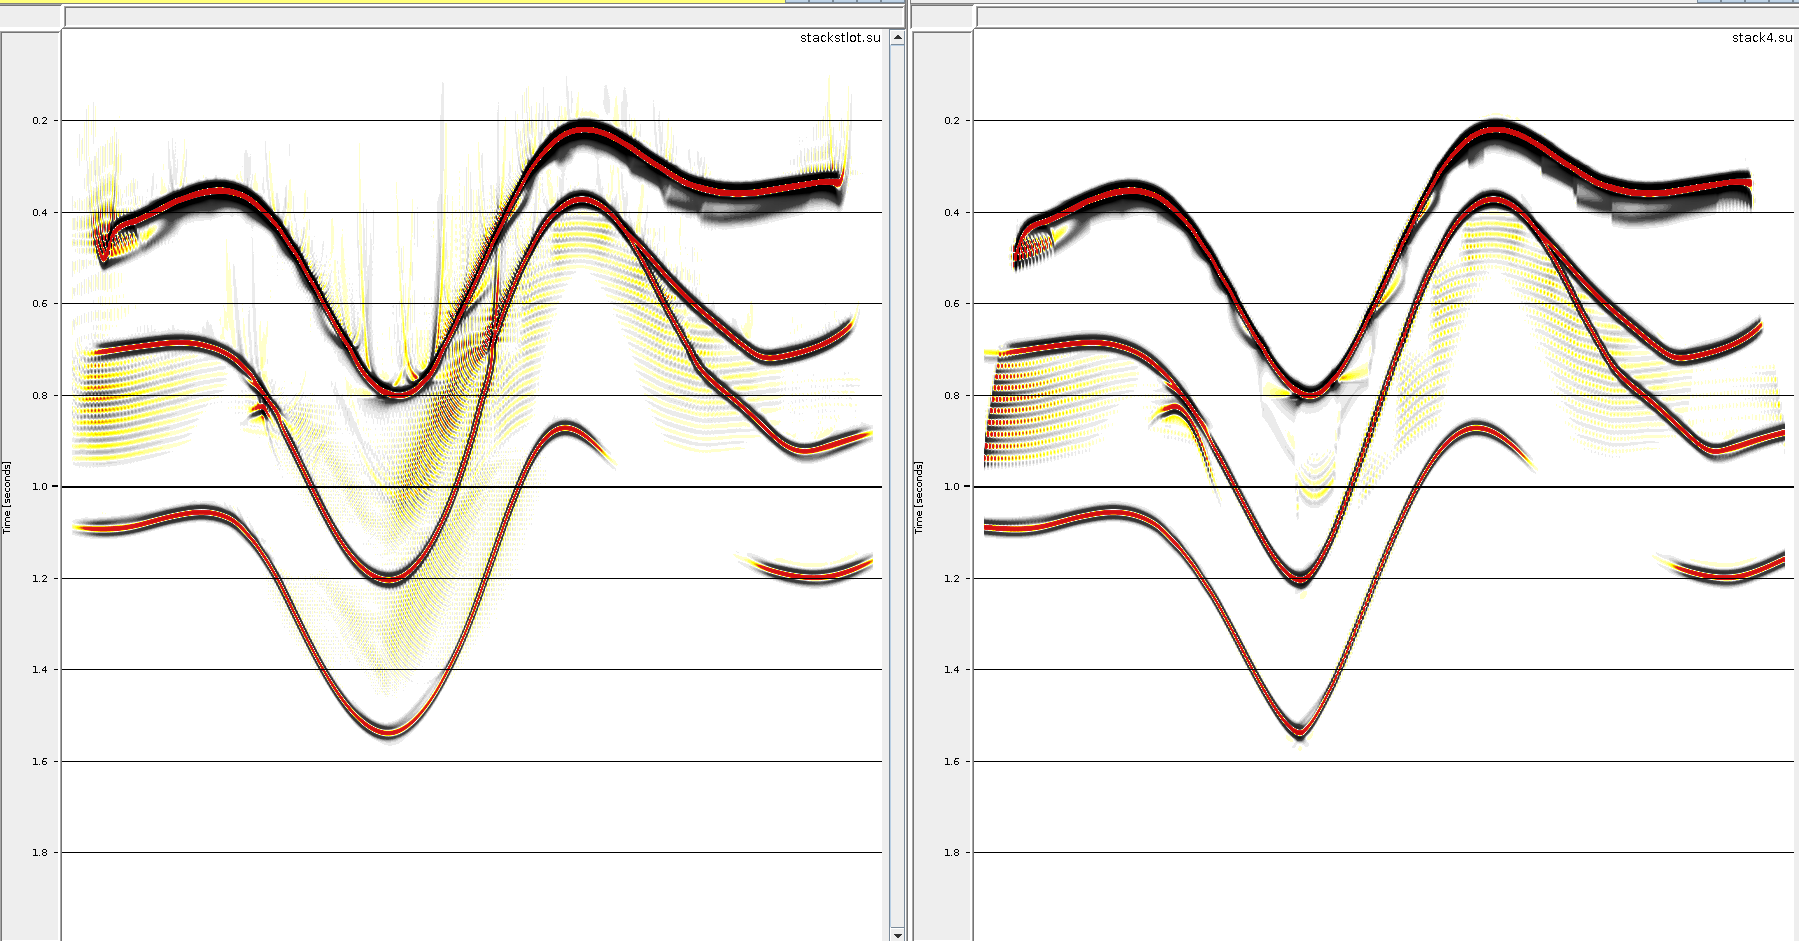
\includegraphics[bb=0 0 1295 678,scale=.25]{SU/fig/stoltmig.png}
	\caption{sustlot偏移}
	\label{fig:sustlot}
\end{figure}

	\chapter{实际地震资料处理}

\section{道充零 sukill} 
\begin{lstlisting}
sukill < $indata min=61 count=2
\end{lstlisting}
道充零没有关键字,通过数道得到他们。

\section{f-x显示}
suspecf制作fx频谱图,suop op=norm归一化操作
\begin{lstlisting}
# Create frequency spectrum of each trace and normalize
suspecfx < $indata | suop op=norm |
# Plot frequency traces
suximage xbox=10 ybox=10 wbox=400 hbox=600 label1=" Freq (Hz)" windowtitle="f-x spectrum" title=$indata cmap=hsv7 legend=1 unit=Amplitude verbose=0 bclip=0.5 wclip=0.0 
\end{lstlisting}
交互脚本见附件fxdisp.sh

\section{滤波、重采样抽道集}
滤波sufilter例子:
\begin{lstlisting}
#Examples of filters:							
Bandpass:   sufilter <data f=10,20,40,50 | ...			
Bandreject: sufilter <data f=10,20,30,40 amps=1.,0.,0.,1. | ..	
Lowpass:    sufilter <data f=10,20,40,50 amps=1.,1.,0.,0. | ...	
Highpass:   sufilter <data f=10,20,40,50 amps=0.,0.,1.,1. | ...	
Notch:      sufilter <data f=10,12.5,35,50,60 amps=1.,.5,0.,.5,1. |..	

sufilter < $indata f=16,21,85,95 amps=0,1,1,0 | 
suresamp nt=2750 dt=.004 | susort > $outdata cdp offset
\end{lstlisting}

\section{球面补偿}
球面补偿简单的应用,已分贝形式查看比较补偿前后的变化。:
\begin{lstlisting}
sugain < indata.su tpow=2 > outdata.su
suwind < $indata key=$mykey min=$mykey1 max=$mykey2 | suattributes mode=amp | suop op=db > tmp0
\end{lstlisting}
\par
理论上球面扩散是1/(距离)的平方,但实际上不是需要进行不同的尝试。\par
交互界面能量补偿见igain.sh。\par

\section{单道处理与多道处理区别}
单道处理不用考虑临近道的关系,例如在炮集中和cmp道集中进行处理结果都是一样的。\par
多道处理则是必须考虑道临近道之间的关系。\par
\begin{tabular}{ll}
\toprule
Single-trace & Multi-trace\\
\midrule
sugain – gain & sunmo – NMO\\
sufilter – 1-D filter & sukill – kill trace\\
suvelan – semblance & sudipfilt – 2-D filter\\
supef – deconvolution & sustolt – Stolt migration\\
\bottomrule
\end{tabular}\par

\section{F-K滤波}
$F-K$滤波通过sudipfilt来实现,$F-K$滤波的斜率可以用相对单位(seconds/meter)或者是绝对单位(number of samples)\par
\begin{tabular}{|lll|}
	\toprule
 a pass filter &  slopes=s1,s2,s3,s4  &  amps=0,1,1,0\\

a reject filter  &  slopes=s1,s2,s3,s4  &  amps=1,0,0,1\\
\bottomrule
\end{tabular}\par\mvspace\mvspace
suspecfk查看分析地震数据的频谱:
\begin{lstlisting}
suspecfk < indata.su dx=$dx dt=$dt | suximage xbox=320 ybox=10 wbox=300 hbox=500 \
label1=" Frequency (Hz)" label2="Wavenumber (k)" title="f-k spectrum, no filter"  cmap=hsv2 legend=1 units=Amplitude verbose=0 grid1=dots grid2=dots perc=99 &
\end{lstlisting}
indata.su为需要进行f-k变化的一炮地震数据
\begin{lstlisting}
#通过的数据
sudipfilt < tmp1 dx=$dx dt=$dt slopes=$slopes amps=0,1,1,0 > tmp2
# Plot f-k passed data
suspecfk < tmp2 dx=$dx dt=$dt | 
suximage xbox=320 ybox=10 wbox=300 hbox=500 label1=" Frequency (Hz)" label2="Wavenumber (k)" title="f-k Spectrum after PASS filter" cmap=hsv2 legend=1 units=Amplitude verbose=0 grid1=dots grid2=dots perc=99 &
# Apply reject filter
sudipfilt < tmp1 dx=$dx dt=$dt slopes=$slopes amps=1,0,0,1 > tmp3
# Plot f-k rejected data
suspecfk < tmp3 dx=$dx dt=$dt |
suximage
xbox=940 ybox=10 wbox=300 hbox=500 label1=" Frequency (Hz)" label2="Wavenumber (k)" title="f-k Spectrum after REJECT filter" cmap=hsv2 legend=1 units=Amplitude verbose=0 grid1=dots grid2=dots perc=99 &
\end{lstlisting}

\section{反褶积}
反褶通过压缩子波波形来提高提高时间分辨率。\par
supef (Wiener predictive error filtering)反褶积两个重要的参数是 minlag (seconds)[prediction length] 和 maxlag (seconds)[ operator length]. 
supef parameter pnoise: the percent white noise 白噪音\par
Operator length 一定要大于 prediction length.\par
另个程序suacor画的是每一道的自相关,用来分析反褶积的一个重要工具\par
supef有关于自相关窗口大小的参数设置,而suacor没有自相关窗口参数。\par

\subsection{反褶积前先进行自相关,跟反褶积之后的结果进行对比}
\begin{lstlisting}
#时间截断
suwind < tmp1 tmin=$taa tmax=$tzz > tmp2
#自相关
suacor < tmp2 ntout=101 sym=0 |
suxwigb perc=$myperc xbox=322 ybox=10 wbox=300 hbox=500 label1=" Time (s)" label2=$mykey key=$mykey windowtitle="Acor before decon" title="Autocorrelation" wclip=0 verbose=0 &
\end{lstlisting}

\subsection{反褶积}
\begin{lstlisting}
# Deconvolution
supef < tmp1 minlag=$minlag maxlag=$maxlag mincorr=$taa maxcorr=$tzz pnoise=$wnoise > tmp3
\end{lstlisting}

\subsection{反褶积之后自相关}
\begin{lstlisting}
suwind < tmp3 tmin=$taa tmax=$tzz > tmp4
suacor <tmp4 ntout=101 sym=0 |
suxwigb perc=$myperc xbox=946 ybox=10 wbox=300 hbox=500 label1=" Time (s)" label2=$mykey key=$mykey title="Acor: first time = $taa, last time = $tzz"  windowtitle="Acor after decon" verbose=0 &
\end{lstlisting}

\subsection{先增益还是先滤波}
\begin{lstlisting}
sudiff T5kgf820.su T5kfg820.su > Tdiff820.su
sudiff T5kgf930.su T5kfg930.su > Tdiff930.su
\end{lstlisting}
不知道哪一个更好,需要进行比较,看实际情况而定


	\part{Madagascar}
	
\end{document}